% !TeX root = ../my-thesis.tex
\chapter{Energieeffizientes Multithreading}

\section{Darstellung der Messwerte}

In diesem Kapitel werden die Ergebnisse der Messungen für die Untersuchung des Zusammenhangs zwischen Multithreading und der Energieeffizienz vorgestellt. Für diese Untersuchung wurden insgesamt 16 Messungen der Ausführung des Base64-Encoders mit steigender Anzahl von Threads unternommen. Die letzte Messung wurde mit 16 Threads durchgeführt. Dies entspricht der doppelten Anzahl an vorhanden physischen Rechenkernen des verwendeten Gerätes. Um den Zeitrahmen dieser Untersuchung nicht zu sprengen, wurden keine Messungen mit einer noch größeren Anzahl von Threads durchgeführt. An dieser Stelle sei gesagt, dass trotz der Begrenzung auf 16 Threads eine klare Tendenz zu erkennen ist, welche weitere Messungen überflüssig machen könnte.

In \autoref{tab:Base64Laufzeit} sind zunächst die ermittelten Laufzeiten der Ausführungen mit steigender Anzahl von Threads zu sehen. Es ist erkennbar, dass bis zu der Marke von 11 Threads ein stetiger Zuwachs an Ausführungsgeschwindigkeit zu erkennen ist, da die Laufzeit bis zu diesem Punkt konstant abnimmt. Zwar ist die Ausführung ab 12 Threads immer noch performanter als ursprünglich, verliert jedoch mit wachsender Anzahl an Threads allmählich an Geschwindigkeit.

% Table generated by Excel2LaTeX from sheet 'Tabelle1'
\begin{table}[htbp]
  \centering
  \caption{Laufzeit in Abh\"angigkeit von der Thread Anzahl}
    \begin{tabular}{rrrr}
    \toprule
    \multicolumn{1}{c}{Threads} & \multicolumn{1}{c}{t in ms} & \multicolumn{1}{l}{Speedup} & \multicolumn{1}{l}{Effizienz} \\
    \midrule
    1     & 994358 & 1,000 & 1,000 \\
    \midrule
    2     & 631836 & 1,574 & 0,787 \\
    \midrule
    3     & 507871 & 1,958 & 0,653 \\
    \midrule
    4     & 441615 & 2,252 & 0,563 \\
    \midrule
    5     & 416036 & 2,390 & 0,478 \\
    \midrule
    6     & 387519 & 2,566 & 0,428 \\
    \midrule
    7     & 369424 & 2,692 & 0,385 \\
    \midrule
    8     & 364560 & 2,728 & 0,341 \\
    \midrule
    9     & 364637 & 2,727 & 0,303 \\
    \midrule
    10    & 355893 & 2,794 & 0,279 \\
    \midrule
    11    & 355677 & 2,796 & 0,254 \\
    \midrule
    12    & 364313 & 2,729 & 0,227 \\
    \midrule
    13    & 363055 & 2,739 & 0,211 \\
    \midrule
    14    & 377380 & 2,635 & 0,188 \\
    \midrule
    15    & 383928 & 2,590 & 0,173 \\
    \midrule
    16    & 395553 & 2,514 & 0,157 \\
    \bottomrule
    \end{tabular}%
  \label{tab:Base64Laufzeit}%
\end{table}%


In \autoref{fig:Base64LeistungPic} ist ein Diagramm dieser Entwicklung zu sehen. Da im Testgerät acht physische Rechenkerne verbaut sind kan das das Gerät nur bis zu acht Threads wirklich parallel bearbeiten. Ab der Marke von neun Threads, ist die \ac{cpu} gezwungen ständig zwischen den Threads hin und her zu wechseln. Diese Art der Ausführung ist zwar noch nebenläufig aber nicht vollständig parallel. Bei jedem Kontextwechsel, muss der Status der Ausführung des aktuellen Threads gespeichert werden sodass die \ac{cpu} später an der richtigen Stelle mit der Berechnung fortfahren kann. Das Speichern und Laden der Register- und Prozessinformationen bei solch einem Kontextwechsel fordert Rechenaufwand und Zeit \cite[2]{MultiThreadingThesis}. Mit steigender Anzahl von Threads verstärkt sich dieser Effekt. Nun könnte die Annahme getroffen werden, dass aus diesem Grund die optimale Thread-Anzahl gleich der Anzahl an physischen Threads ist. Dies würde im Fall des hier verwendeten Gerätes bedeuten, dass acht Threads die schnellste Laufzeit erreichen müssten. Es ist jedoch zu erkennen, dass die Ausführung mit 11 Threads das beste Ergebnis liefert. Hierbei wurde mit 355677 \ac{ms} 63,3 \% weniger Laufzeit benötigt als mit einem Thread. Mit acht Threads hingegen sind es mit 364560 \ac{ms} nur 63,3 \% weniger. Eine weitere Auffälligkeit ist der massive Geschwindigkeitszuwachs bei dem Übergang von einem Thread zu zwei Threads. Der Speedup $S_{p}(2)$ nach \autoref{eq:Amdahlsche Gesetz} beträgt 1,57 und die daraus ermittelte Laufzeiteffizienz für zwei Threads $E_{ p }(2)$ nach \autoref{eq:Effizienz} beträgt 0,79 \todo{speedup und Effizienz in tagbelle ergänzen }. Statt den ursprünglichen 994358 \ac{ms} mit einem Thread benötigt die Kodierung mit zwei Threads nur noch 631836 \ac{ms} bis zur Terminierung. Das entspricht einer Laufzeitverringerung von  36,5 \%. Nach der Zuschaltung von Thread 3 beträgt die Laufzeit 507871 \ac{ms}. Das sind nur 12,4 \% weniger als die Kodierung mit zwei Threads. Die Laufzeiteffizienz $E_{ p }(3)$ beträgt nur noch 0,65. 

Hierfür gibt es zwei Hauptgründe. Der massive Performancezuwachs bei der Nutzung von zwei Threads ist mit der Exynos 7885 \ac{soc}-Architektur der \ac{cpu} des verwendeten Gerätes zu erklären. Diese Architektur kombiniert zwei leistungsstarke Cortex-A73 Rechenkerne mit jeweils 2,20 \ac{ghz} Taktrate und vier energiesparende Cortext-A53 Kerne mit jeweils 1,60 \ac{ghz} Taktrate. Bei der Nutzung von zwei Threads, wird zunächst der Cortex-A73 zugeschaltet. Danach stehen ausschließlich die restlichen Cortex-A53 Kerne zur Verfügung, welche mit ihrer geringeren Taktrate natürlich auch einen geringeren Speedup $S_{p}(n)$ liefern. Die Tatsache, dass die Ausführungsgeschwindigkeit bis zu der Marke von 11 Threads ansteigt, obwohl nur acht physische Kerne vorhanden sind, ist ebenfalls mit der Exynos 7885 \ac{soc}-Architektur zu begründen. Ab der Marke von neun Threads, werden mehr \emph{Callables} bearbeitet als physische Kerne vorhanden sind. Das bedeutet, dass ab neun Threads Kontextwechsel durchgeführt werden müssen um alle Threads mit Rechenzeit zu bedienen. Da trotz Dessen bessere Laufzeiten bis zur Marke von 11 Threads zustande kommen, liegt die Vermutung nahe, dass die beiden Cortex-A73 Rechenkerne aufgrund ihrer höheren Rechenleistung für die Kontextwechsel priorisiert werden und daher letztendlich mehr Anteile der Kodierung durchführen. In der Implementierung des Base64-Encoders werden die einzelnen Aufgabenpakte für die Threads so vergeben, dass jedes Aufgabenpaket (\emph{Callable}) die gleiche Textmenge kodiert. Die beiden Cortex-A73 Rechenkerne sind aufgrund ihrer höheren Taktrate natürlich schneller mit ihrem Aufgabenpaket fertig als die andern Kerne. Somit befinden sich die Cortex-A73 Rechenkerne bis zu der Marke von acht Threads im Leerlauf, sobald sie ihre Aufgabenpakete abgearbeitet haben. Ab der Nutzung von weiteren Threads kommt es nicht mehr zu diesen Leerlaufzeiten, da durch den Kontextwechsel die Bearbeitung von mehreren Arbeitspaketen  möglich wird. Der prozentuale Anteil an durch die Cortex-A73 Rechenkerne kodierte Text steigt also ab der neun Thread-Marke. Die bessere Auslastung der beiden schnellen Rechenkerne relativiert bis zur Marke von 11 Threads den Zeitaufwand für die Kontextwechsel und führt zu einer schnelleren Laufzeit. Ab der Marke von 12 Threads nimmt der Aufwand für die Kontextwechsel zwischen den vielen Threads allerdings so stark zu, dass der Speedup allmählich sinkt und die Laufzeitkosten wieder steigen. 

\begin{figure}[H]
	\begin{center}	 
	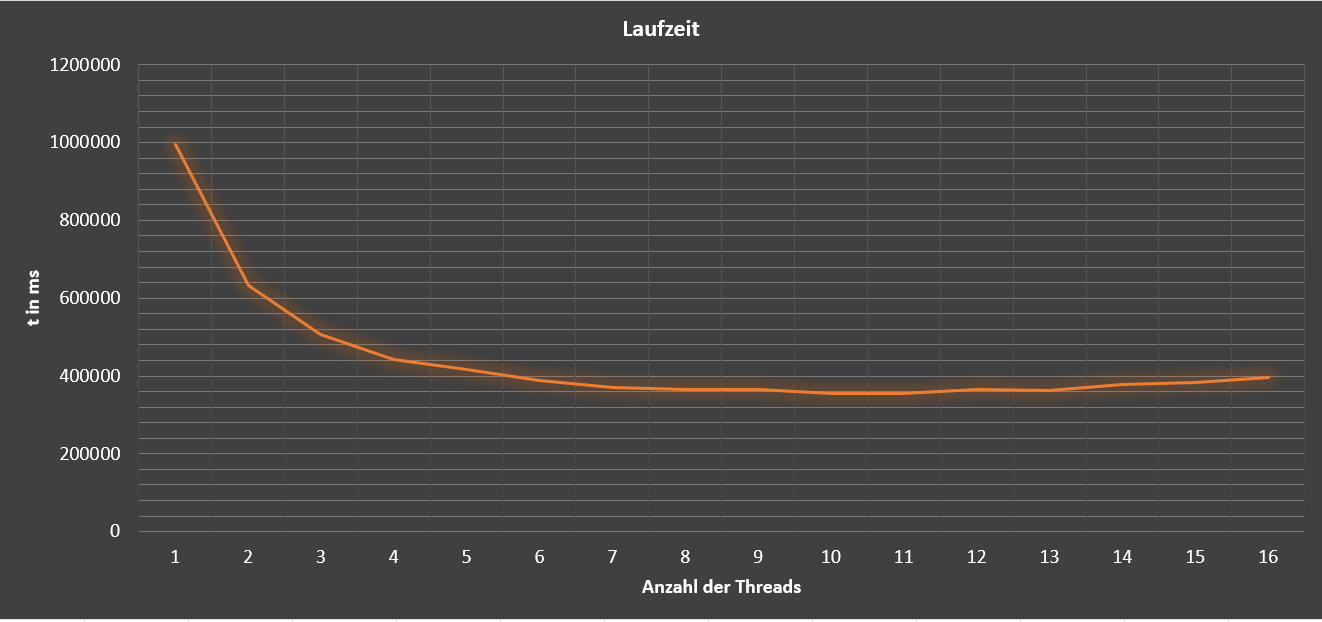
\includegraphics[width=0.8\textwidth]{Base64LaufzeitPic}
	\caption{Laufzeitdiagramm (eigene Abbildung)}
	\label{fig:Base64LaufzeitPic} 
	\end{center}
\end{figure}


% !TeX root = ../my-thesis.tex
% Table generated by Excel2LaTeX from sheet 'Tabelle1'
\begin{table}[htbp]
  \centering
  \caption{durchschnittliche Leistungsaufnahme in Abh\"angigkeit von der Thread Anzahl}
    \begin{tabular}{rrrr}
    \toprule
    \multicolumn{1}{c}{Threads} & \multicolumn{1}{c}{\O U in mV} & \multicolumn{1}{c}{\O I in mA} & \multicolumn{1}{c}{\O P in W} \\
    \midrule
    1     & 4077,382 & 565,944 & 2,306 \\
    \midrule
    2     & 3997,636 & 733,983 & 2,931 \\
    \midrule
    3     & 4029,556 & 860,404 & 3,462 \\
    \midrule
    4     & 4056,719 & 859,178 & 3,479 \\
    \midrule
    5     & 4043,867 & 869,086 & 3,505 \\
    \midrule
    6     & 4028,429 & 900,618 & 3,621 \\
    \midrule
    7     & 4017,545 & 923,407 & 3,705 \\
    \midrule
    8     & 4042,727 & 933,792 & 3,772 \\
    \midrule
    9     & 4063,227 & 901,938 & 3,662 \\
    \midrule
    10    & 4046,045 & 934,489 & 3,775 \\
    \midrule
    11    & 4034,455 & 948,283 & 3,824 \\
    \midrule
    12    & 4074,458 & 856,408 & 3,485 \\
    \midrule
    13    & 4049,000 & 962,385 & 3,486 \\
    \midrule
    14    & 4063,917 & 915,918 & 3,586 \\
    \midrule
    15    & 4021,708 & 926,291 & 3,726 \\
    \midrule
    16    & 4023,542 & 946,001 & 3,806 \\
    \bottomrule
    \end{tabular}%
  \label{tab:Base64Leistung}%
\end{table}%


\begin{figure}[h]
	\begin{center}	 
	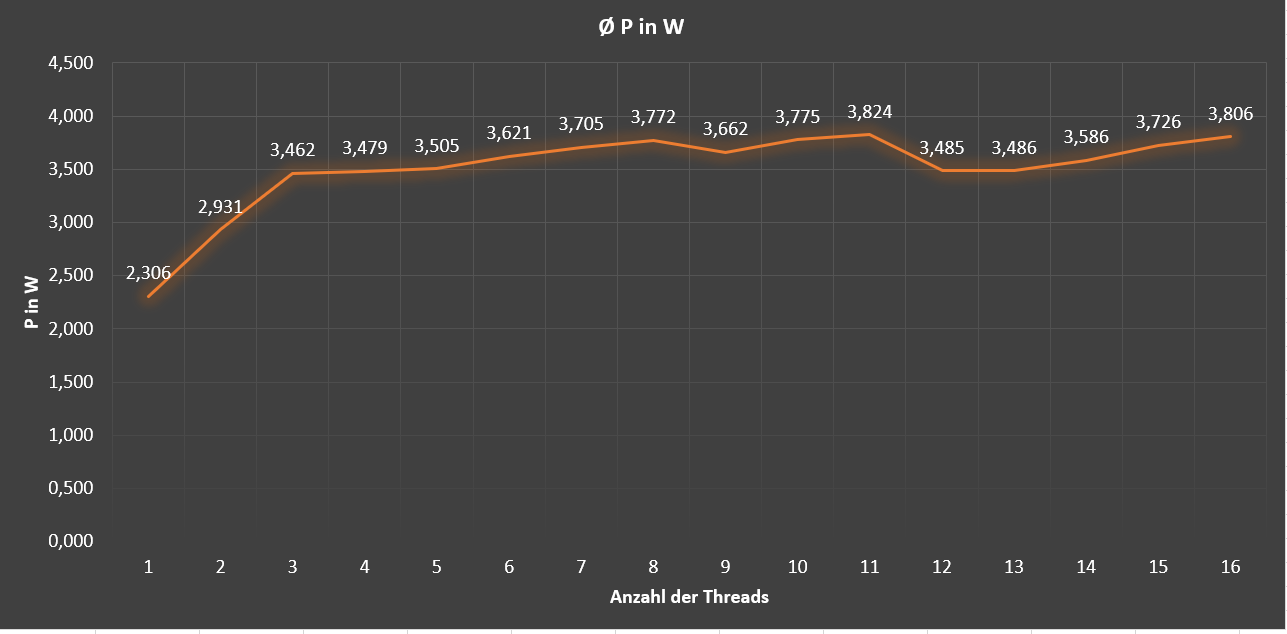
\includegraphics[width=0.8\textwidth]{Base64LeistungPic}
	\caption{durchschnittliche elektrische Leistung in Abhängigkeit von der Thread Anzahl (eigene Abbildung)}
	\label{fig:Base64LeistungPic} 
	\end{center}
\end{figure}

% !TeX root = ../my-thesis.tex
% Table generated by Excel2LaTeX from sheet 'Tabelle1'
\begin{table}[htbp]
  \centering
  \caption{elektrische Arbeit in Abhängigkeit von der Thread Anzahl}
    \begin{tabular}{rr}
    \toprule
    \multicolumn{1}{c}{Threads} & \multicolumn{1}{c}{W in Ws} \\
    \midrule
    1     & 2330,170 \\
    \midrule
    2     & 1891,658 \\
    \midrule
    3     & 1815,574 \\
    \midrule
    4     & 1594,628 \\
    \midrule
    5     & 1532,691 \\
    \midrule
    6     & 1473,056 \\
    \midrule
    7     & 1347,732 \\
    \midrule
    8     & 1296,977 \\
    \midrule
    9     & 1252,836 \\
    \midrule
    10    & 1290,069 \\
    \midrule
    11    & 1306,284 \\
    \midrule
    12    & 1316,109 \\
    \midrule
    13    & 1322,537 \\
    \midrule
    14    & 1374,502 \\
    \midrule
    15    & 1393,833 \\
    \midrule
    16    & 1409,848 \\
    \bottomrule
    \end{tabular}%
  \label{tab:Base64Arbeit}%
\end{table}%


\begin{figure}[H]
	\begin{center}	 
	\includegraphics[width=0.95\textwidth]{Base64LeistungFlächePic}
	\caption{Verlauf der elektrischen Leistung mit einem Thread (eigene Abbildung)}
	\label{fig:Base64LeistungFlächePic} 
	\end{center}
\end{figure}

\begin{figure}[H]
	\begin{center}	 
	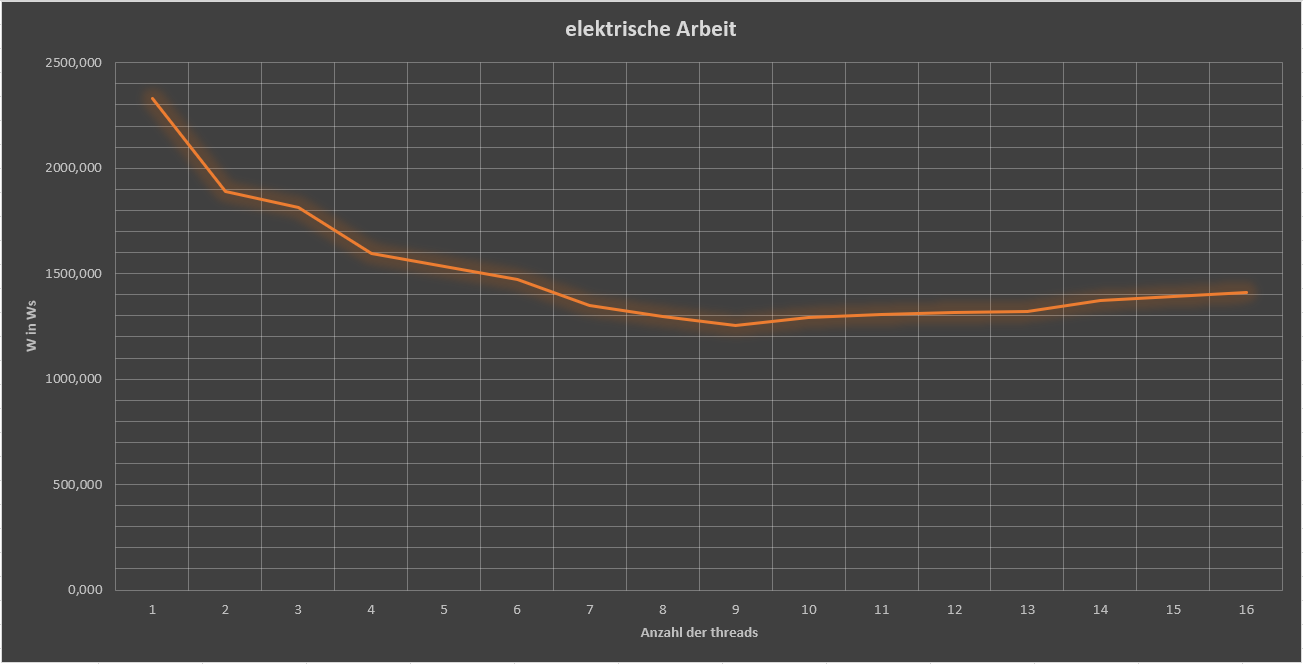
\includegraphics[width=0.95\textwidth]{Base64ArbeitPic}
	\caption{elektrische Arbeit in Abhängigkeit der Thread Anzahl(eigene Abbildung)}
	\label{fig:Base64ArbeitPic} 
	\end{center}
\end{figure}


\section{Auswertung}